% The Models
\documentclass[../main]{subfiles}

\graphicspath{{figures/}{../figures/}}

\begin{document}
\subsection{Fast Response Model}
To discuss the possible deployment of drones in order to detect fire and transmit the signal to EOC,
 we design Fast Response Model to maximize coverage and minimize the cost. To represent the fire distribution,
  fire frequency and fire size, we come up with several well-designed indices and use fire location in certain
   period to represent those factors with minimum lost of information.  Since it's not economically
    efficient to cover all the land of Victoria because the drones are able to move and the fact that fire can
     spread and then be detected, we use weighted covering lost(WCL) to represent the cost for not covering 
     all the possible locations of fire. We use the data in 2020 for case study, but the strategy we adapt and
      the data we compute is generic and can be used in various situation. \\

      After sensitivity test, we proved the robustness of the model. It can be showed that the Fast Response Model can be used in different size of fire, different frequency of fire, and different distribution of fire in state of Victoria and other places in the world.
\subsubsection{Data Pre-processing}
For the sake of CFA, our model should only be considering the fire situation within the range of state of Victoria. The data we obtained from NASA database is contains noise and locations out of border. The first step of data pre-processing is meant to sift out all the illegal point with criteria mentioned above. Considering the spatial location of noise point,
 we use DBSCAN clustering with ball tree \cite{enwiki:1065597644} algorithm, and is implemented by sci-learn 
 project\cite{scikit-learn}. 
 Since the data contains latitude and longitude, 
 to define the distance function for clustering one need to use the haversine formula\cite{haversine} to calculate the great-circle distance between two points.
 


 \begin{equation}
      dist_{i,j}=2\cdot R_{e} \cdot \arctan \Bigg(\sqrt{\frac {\sin^2(\frac {\Delta \varphi_{lat} }{2})+\cos\varphi _i\cdot 
      \cos \varphi _j \cdot \sin^2({ \frac {\Delta \lambda_{lon}} {2} })}
      {1-(\sin^2(\frac {\Delta \varphi_{lat} }{2})+\cos\varphi _i\cdot 
      \cos \varphi _j \cdot \sin^2({ \frac {\Delta \lambda_{lon}} {2} }))}}\Bigg)
\end{equation}

This ensures the correctness of clustering.

To define a noise point which is inefficient to cover it, we define two
variables \(eps\) and \(minPoints\) according to DBSCAN conventions.

To more easily obtain the optimized value, we first normalize data with
standard normalization, then we set

\begin{equation}
      \left\{
      \begin{array}{l}
            eps=0.15\\
            minPoints=8
      \end{array}
      \right.
\end{equation}

\begin{figure}[h!]
  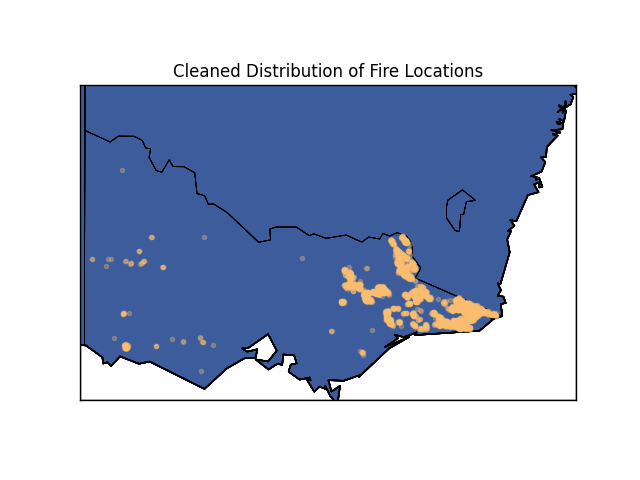
\includegraphics[width=\linewidth]{no_clustering.png}
  \caption{Cleaned Fired Distribution}
  % \label{fig:boat1}
\end{figure}

\subsubsection{Deploying SSA}

To deploy drones in a way that reaches the target of fast response, we
first need to quantify the target using one index, which we define it as
weighted covering lost(WCL).

\begin{equation}
WCL=\sum_j \Bigg(\int _{x0} ^{x1}  { (x-r_c)\cdot (1-p_{j,x})} \cdot vs_{j,x} \Bigg) \  dx \\ \\
\end{equation}

To simplify our model, we assume \(vs_{j,x}=v\), which is a stable
value, then we have.

\begin{equation}
WCL=\sum_j \Bigg(\int _{x0} ^{x1}  { (x-r_c)\cdot p_{j,x}} \cdot  v  \  dx\Bigg)^2
\end{equation}

In order to simply the model as well as simulate the distribution of
\(p_{j}\), we use Ridge Distribution to set \(p_{j,x}\), which is the
probability of rim of fire at the position which is \(x\) km from the
nearest SSA, as following

\begin{equation}
p_{j,x}=
\begin{cases}
\frac 1 2 - \frac 1 2 \sin \frac {\pi} {r_o}(x-\frac {r_o} {2} ) , & 0\le x \le r_0 \\ 
0 , & x > r_0
\end{cases}  
\end{equation}

This gives us

\begin{equation}
WCL=\sum_j \Bigg(\int _{x0} ^{x1}  { (x-r_c)\cdot (\frac 1 2 + \frac 1 2 \sin \frac {\pi} {r_o}(x-\frac {r_o} {2} ))} \cdot  v  \  dx \Bigg)^2
\end{equation}

We use the concept of substitution distance(\(sdist\)) to investigate
the deployment strategy.

\begin{equation}
sdist=\Bigg\| \int _{x0} ^{x1}  { (x-r_c)\cdot (\frac 1 2 + \frac 1 2 \sin \frac {\pi} {r_o}(x-\frac {r_o} {2} ))} \cdot  v  \  dx \Bigg\|
\end{equation}

We define \(sdist\) in a way that guarantees \(sdist\) is positively
correlated to \(x\) which is the distance to the center, that is, the
place where the nearest drone is deployed.

To balance economical costs and safety, we set a threshold for \(WCL\),
\(tWCL\) which is currently set to a certain value in our later
investigation, but it can be adjusted according to real situation. It
will be illustrated more thoroughly in the following section about
sensitivity and robustness. We use modified \(k-means\) cluster to
determine the positions of SSAs, which is described as follows

\begin{figure}[h!]
      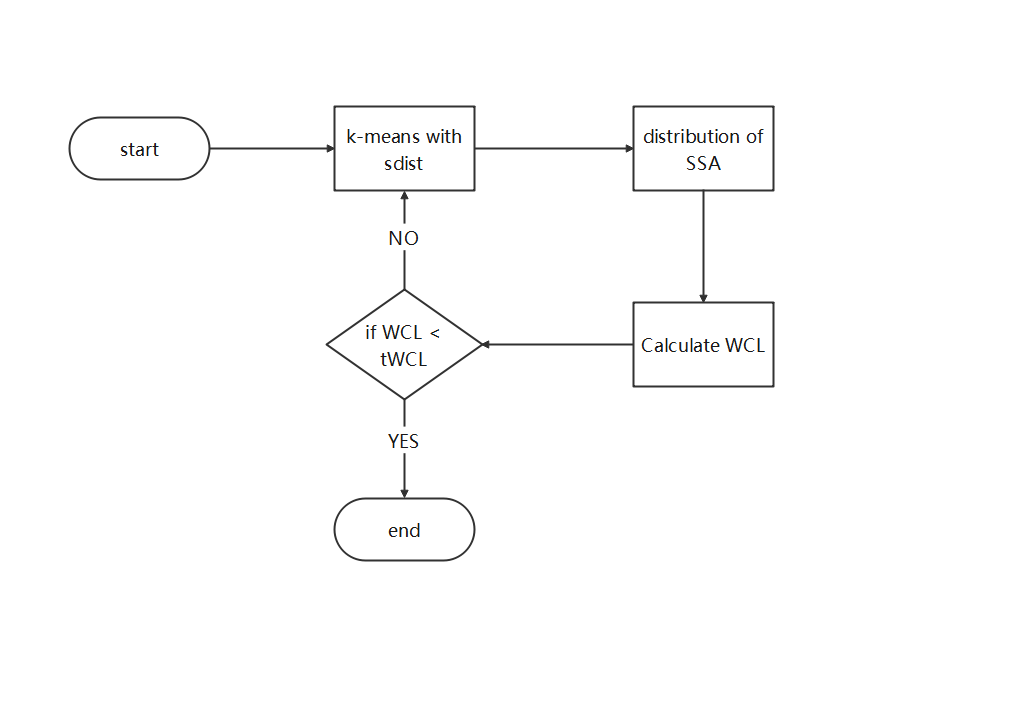
\includegraphics[width=\linewidth]{FlowChart2.png}
      \caption{deploy SSA flowchart}
      % \label{fig:boat1}
    \end{figure}

This allows us to cluster the locations to their respective drones.
k-means algorithm is used here since the \(sdist\) is positively
correlates to distance. So the correctness of the algorithm can be
ensured.



\begin{figure}[h!]
      \centering
      \begin{subfigure}[b]{0.4\linewidth}
        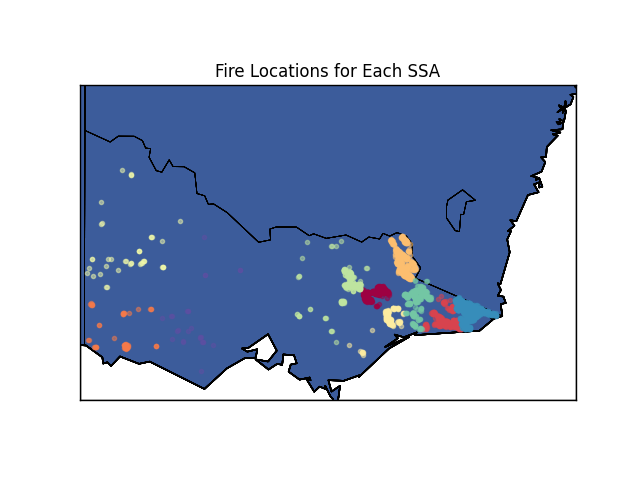
\includegraphics[width=\linewidth]{K-means_clustering.png}
        \caption{clustering of fire location}
      \end{subfigure}
      \begin{subfigure}[b]{0.4\linewidth}
        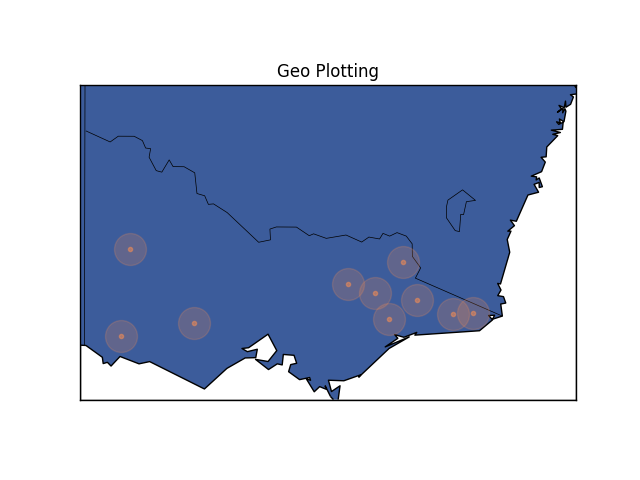
\includegraphics[width=\linewidth]{thermal_drones_deployment.png}
        \caption{SSA distribution}
      \end{subfigure}
      \caption{SSA and fire locations}
      \label{fig:coffee}
    \end{figure}

Given the fire location distribution, we plot the SSA's location as
above. The range is marked as well. It can be observed that the fire is
frequent and in large scale at the east of state of Victoria. Our
distribution perfectly fit the situation can reduce \(WCL\) to
acceptable level.

\subsubsection{Deploy Repeaters}

The second part of Fast Response Model is connecting all the SSAs using
the least repeaters. We solve this problem by divide and conquer and
with the help of minimum spanning tree.

For Dense Cluster, we choose to shrink several SSAs into one, since when
it's dense, one repeater can cover multiple SSAs. Then we build minimum
spanning tree on the repeaters.

For Sparse Cluster, we choose to build minimum spanning tree directly.

Combined both situation, we succeed in connecting all SSAs in a way that
guarantees both the stability of connection and minimum economic cost.

\paragraph{Dense Cluster}

For dense cluster, we choose shrink point strategy. For every dense
cluster which is formed by a set of SSAs, we use an algorithm to settle
the distribution of core repeater.

A core repeater is defined as, the repeater that can receive signal from
SSAs.

\begin{figure}[h!]
      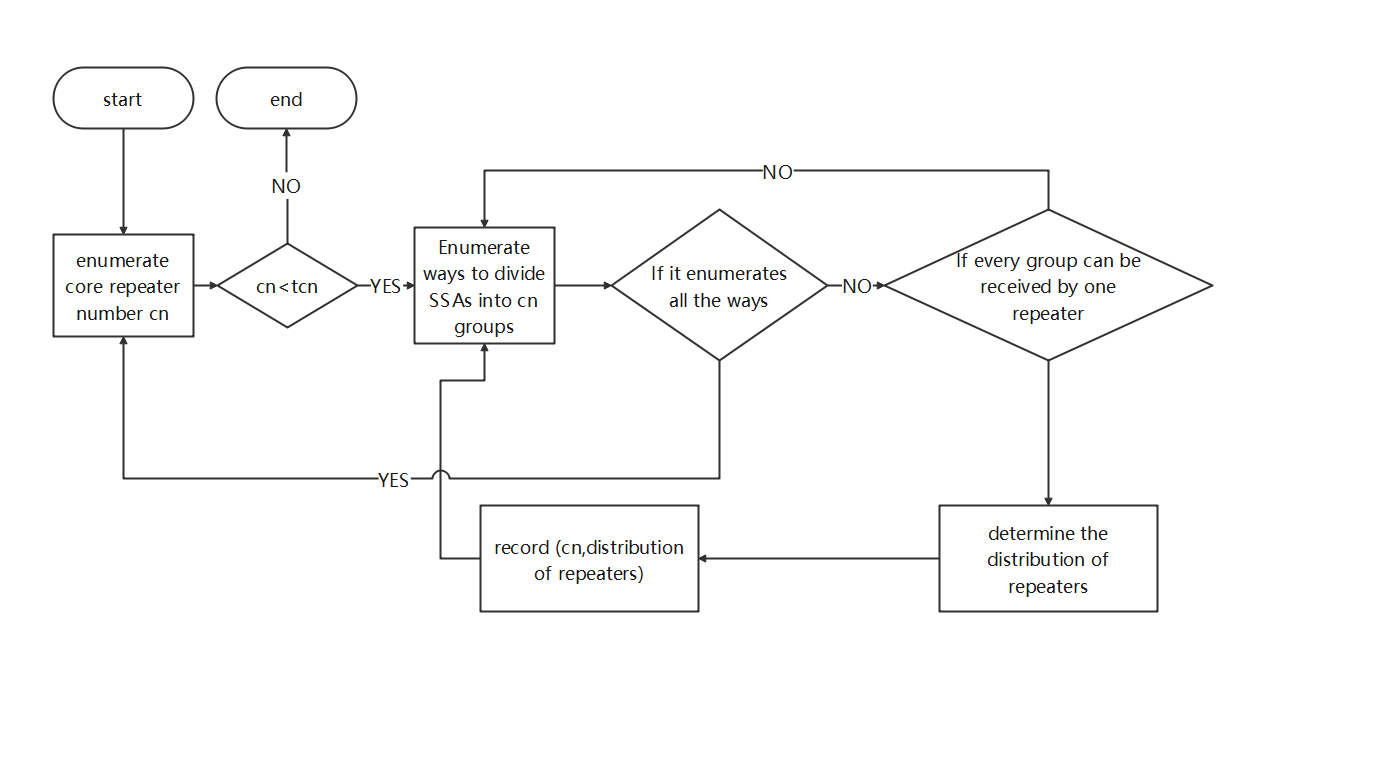
\includegraphics[width=\linewidth]{FlowChart3.png}
      \caption{Strategy for Dense Clutser}
      % \label{fig:boat1}
    \end{figure}

We want the combination of core repeaters to be in a way that allows the
minimum number of repeaters to be distributed and all the SSAs' signal
can be received. There seems to be no elegant solution to this problem
because it is \(NP\) problem. However, the small number of SSAs allows
us to use brute force to compute such distribution.

We define \(cn\) to be the number of core repeaters needed, \(nSSA\) to
be the SSA that are distributed, we define \(tcn\) to be the maximum
number of core repeaters that are allowed, it's obvious that
\(tcn \le nSSA\). For simplicity of implementation, we set \(tcn=nSSA\)

\paragraph{Sparse Cluster and Final Linking}

Now there are only sparse SSAs and sparse repeaters, it's natural to
link them by Kruskal algorithm to make a minimum spanning tree.

The first step is to build the graph with nodes and edges.

\begin{itemize}
\item
  Nodes are SSAs and repeaters, which is reasonable since they are
  sparse and can be discretized.
\item
  Edges have weight defined below. Considering if the range of drones
  are tangent to each other, the transmission stability will be lowered,
  we introduce transmission random factor \(trf\)
\end{itemize}

\begin{equation}
Ew_e= \max{ \Bigg(\Bigg\lceil \frac { dis_{i,j}  - 2r_c - trf_e} {2r_c} \Bigg\rceil,0\Bigg)}
\end{equation}

Transmission factor is defined below to reduce the situation where
ranges of drones are tangent, where \(randi(x)\) function is to randomly
produce a real number within interval \([0,x]\)

\begin{equation}
trf_e= randi \Bigg( 1- \Bigg(\Bigg\lceil \frac { dis_{i,j}  - 2r_c - trf_e} {2r_c} \Bigg\rceil -\frac { dis_{i,j}  - 2r_c - trf_e} {2r_c} \Bigg)\Bigg)
\end{equation}

Then we use Kruskal Algorithm\cite{kruskal} as described below to make a
spanning tree.

\newpage

\begin{figure}[h!]
      \centering
      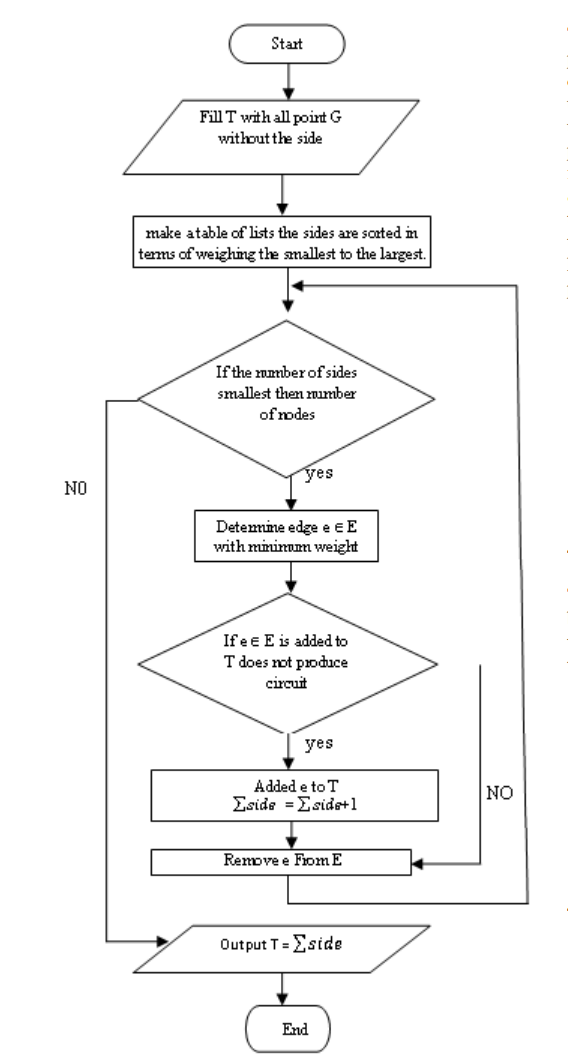
\includegraphics[width=.5\linewidth]{FlowChart4.png}
      \caption{Strategy for Dense Clutser}
      % \label{fig:boat1}
    \end{figure}



\begin{figure}[h!]
      \centering
      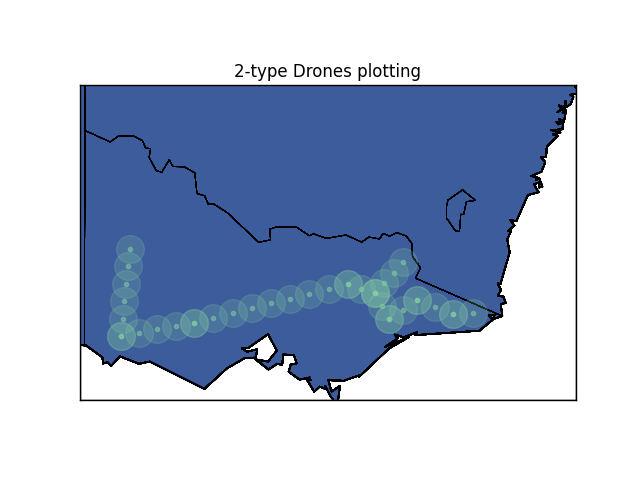
\includegraphics[width=.5\linewidth]{two_type.png}
      \caption{The general drone distribution}
      % \label{fig:boat1}
    \end{figure}

Because of the introduction of \(trf_e\) and the use of divide and
conquer strategy, the outcome is not only stable but also efficient as
shown.
\end{document}
